\documentclass[12pt,a4]{article}




\usepackage{graphicx,amsmath,amssymb,amsthm, boxedminipage,xcolor}

%\usepackage[lined,boxed]{algorithm2e}

\usepackage{algorithm}
\usepackage{algpseudocode}

%\usepackage{algorithmic}
\usepackage{algpseudocode}
\usepackage{amsmath}
\usepackage{graphics}
\usepackage{epsfig}

\newtheorem{theorem}{Theorem}[section]
\newtheorem{proposition}[theorem]{Proposition}
\newtheorem{lemma}[theorem]{Lemma}
\newtheorem{corollary}[theorem]{Corollary}
\newtheorem{definition}[theorem]{Definition}

\newtheorem*{theorem*}{Theorem}
\newtheorem*{lemma*}{Lemma}
\newtheorem*{proposition*}{Proposition}


\newtheorem{exercise}[theorem]{Exercise}
\newtheorem{exerciseD}[theorem]{*Exercise}
\newtheorem{exerciseDD}[theorem]{**Exercise}

\let\oldexercise\exercise
\renewcommand{\exercise}{\oldexercise\normalfont}

%\let\oldexerciseD\exerciseD
%\renewcommand{\exerciseD}{\oldexerciseD\normalfont}

%\let\oldexerciseDD\exerciseDD
%\renewcommand{\exerciseDD}{\oldexerciseDD\normalfont}

\newcommand{\E}{\mathbb{E}}
%\newcommand{\nth}[1]{#1^{\textsuperscript{th}}}
\newcommand{\scalar}[2]{\ensuremath{\langle #1, #2\rangle}}
\newcommand{\floor}[1]{\left\lfloor #1 \right\rfloor}
\newcommand{\ceil}[1]{\left\lceil #1 \right\rceil}
\newcommand{\norm}[1]{\|#1\|}
\newcommand{\pfrac}[2]{\left(\frac{#1}{#2}\right)}
\newcommand{\nth}[1]{#1^{\textsuperscript{th}}}
\newcommand{\core}{\textnormal{core}}



\newif\ifsolution

\solutionfalse

\newcommand{\answer}[1]{
\ifsolution
{\color{blue} #1}
\else
\fi
}



\newcommand{\poly}{\textnormal{poly}}
\newcommand{\quasipol}{\textnormal{quasipol}}
\newcommand{\ssubexp}{\textnormal{stronglySubExp}}
\newcommand{\wsubexp}{\textnormal{weaklySubExp}}
\newcommand{\simplyexp}{\textnormal{E}}
\newcommand{\expo}{\textnormal{Exp}}



\newcommand{\N}{\mathbb{N}}
\newcommand{\nn}{\mathbb{N}_0^n}
\newcommand{\R}{\mathbb{R}}
\newcommand{\Z}{\mathbb{Z}}


\definecolor{darkgreen}{rgb}{0,0.6,0}


\date{}

\title{
  Mathematical Foundations \\of \\Computer Science\\
  \vspace{3mm}
{\normalsize CS 499,	Shanghai Jiaotong University,  Dominik Scheder}
}

\begin{document}

\maketitle

%\begin{quotation}
%  You are welcome to discuss the exercises in the discussion
%  forum. Please take them serious. Doing the exercises is as important
%  than watching the videos.
%
%  I intentionally included very challenging exercises and marked them
%  with one or two ``$*$''. No star means you should be able to solve
%  the exercises without big problems once you have understood
%  the material from the video lecture. One star means it requires 
%  significant additional thinking. Two stars means it is not 
%  unlikely that you will fail to solve them, even once you have understood
%  the material and thought a lot about the exercise. Don't feel bad
%  if you fail. Failure is part of learning.
%
%  This is the first time this course is online. Thus there might be mistakes
%  (typos or more serious conceptual mistakes) in the exercises. I will be 
%  grateful if you point them out to me!
%\end{quotation}





\setcounter{section}{6}

\section{The Graph Score Theorem}



\begin{itemize}
 \item Homework assignment published on Monday, 2018-04-09.
 \item Submit questions and first solution by Sunday, 2018-04-15, 12:00 by
 email to dominik.scheder@gmail.com and the TAs.
 \item You will receive feedback by Wednesday, 2018-04-18.
 \item Submit your final solution by Sunday, 2018-04-22 to me and the two TAs.
\end{itemize}


\begin{exercise}
  Describe, in simple sentences with a minimum of mathematical formalism, (1) the score
  of a graph, (2) what the graph score theorem is, (3) the idea of the 
  graph score algorithm, (4) where the difficult part of its proof is.
  Imagine you have a friend who does not take this class, and think about how to answer
  the above questions to them.
\end{exercise} 




\subsection{Alternative Graphs}

Now we will look at different notions of graphs. As defined in class and in the video
lectures, a graph is a pair $G = (V,E)$ where $V$ is a (usually finite) set, called the {\em vertices},
and $E \subseteq {V \choose 2}$, called the set of {\em edges}.

\paragraph{Multigraphs.} 
A {\em multigraph} is like a graph, but you can have several parallel edges between
two vertices. You cannot, however, have self-loops. That is, there cannot
be an edge from $u$ to $u$ itself. This is an example of a multigraph:

\begin{center}
  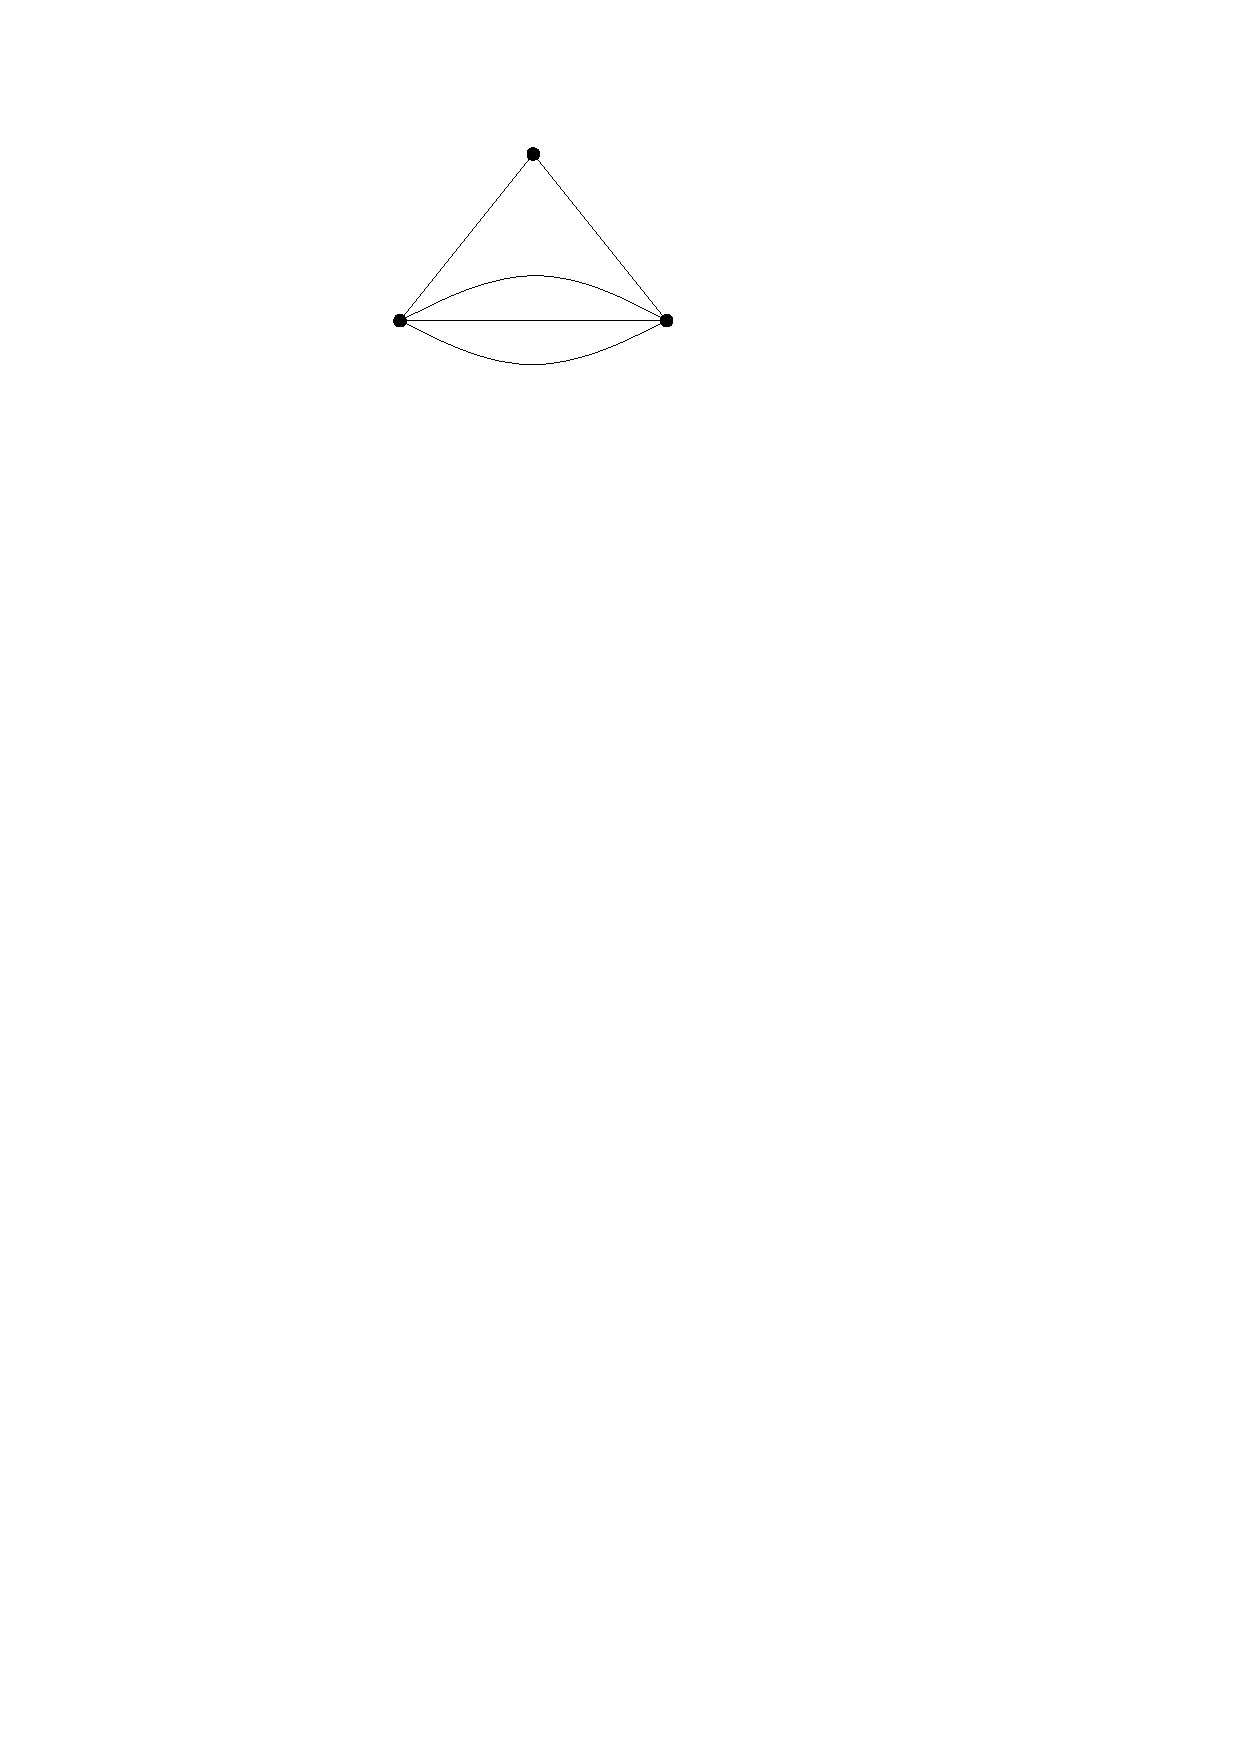
\includegraphics[width=0.25\textwidth]{figures/multigraph-score.pdf}
\end{center}

We can define degree and score for multigraphs, too. For example, this multigraph
has score $(4,4,2)$. Obviously no graph
can have this score.



\begin{exercise}
  State a score theorem for multigraphs. That is, something like
  \begin{theorem}[Multigraph Score Theorem]
     Let $(a_1,\dots,a_n) \in \N_0^n$. There is a multigraph
     with this score if and only if \texttt{\textup{<fill in some simple criterion here>}}.
  \end{theorem}
  
  
  \textbf{Remark.} This is actually
  simpler than for graphs.
\end{exercise}

\begin{exercise}
  Prove your theorem.
\end{exercise}




\newcommand{\wdeg}{\textnormal{wdeg}}

\paragraph{Weighted graphs.} A weighted graph is a graph in which every edge $e$ has a non-negative weight $w_e$.
In such a graph the {\em weighted degree} of a vertex $u$ is $\wdeg(u) = \sum_{ \{u,v\} \in E} w_{\{u,v\}}$.

\begin{center}
  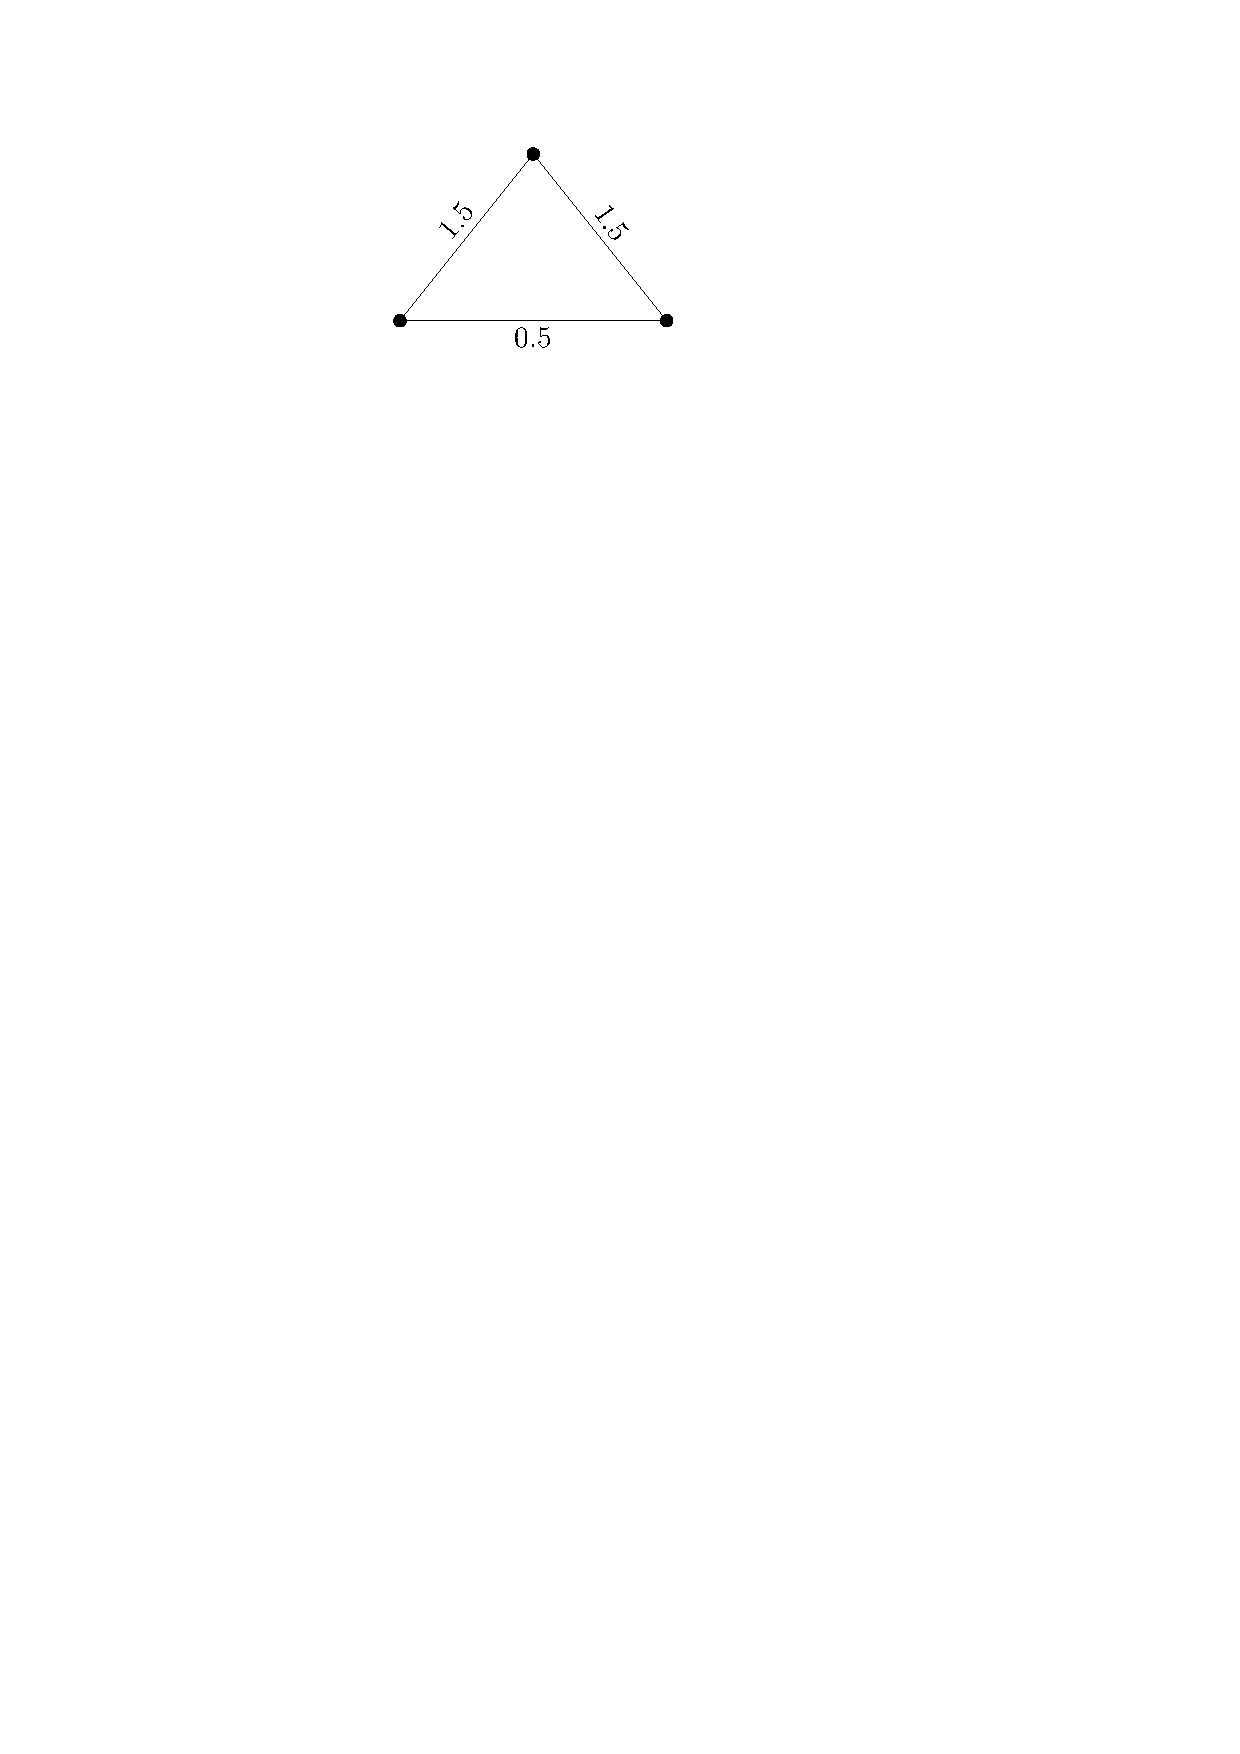
\includegraphics[width=0.25\textwidth]{figures/weighted-graph-score.pdf}
\end{center}

This is an example of a weighted graph, which has score $(3,2,2)$. Obviously no graph
and no multigraph can have this score.


\begin{exercise}
  State a score theorem for weighted graphs. That is, state something like
  \begin{theorem}[Weighted Graph Score Theorem]
     Let $(a_1,\dots,a_n) \in \R_0^n$ $a_1 \geq a_2 \geq \dots \geq a_n$. There is a weighted graph
      with this score if and only if $a_1 \leq a_2 + \dots + a_n$.
  \end{theorem}
  \textbf{Remark.} This 
  is actually even simpler.
\end{exercise}


\begin{exercise}
    \begin{proof}
Suppose $v_1, v_2 , \dots, v_n$ are the corresponding vertices of $a_1, a_2, \dots, a_n$.

Weighted Graph $ \Rightarrow $ $a_1 \leq a_2 + \dots + a_n$

We can split vertices into two groups: $v_1$ and $v_2, \dots, v_n$.

    For each edge $E(u,v)$:

    If $u$ is $v_1$ and $v$ is in $v_2, \dots, v_n$, then $v_1$ gains degree of the weight and $v_2, \dots, v_n$ gain degree of the weight.

    If $u$ is in $v_2, \dots, v_n$ and $v$ is $v_1$, then $v_1$ gains degree of the weight and $v_2, \dots, v_n$ gain degree of the weight.

    If $u$ is in $v_2, \dots, v_n$ and $v$ is $v_2, \dots, v_n$, then $v_1$ gains no degree and $v_2, \dots, v_n$ gain the degree of double weight.

    Therefore, the degree of $v_1$ must be less or equal than the total degree of $v_2, \dots, v_n$, namely $a_1 \leq a_2 + \dots + a_n$.


$a_1 \leq a_2 + \dots + a_n$ $ \Rightarrow $ Weighted Graph

    \textbf{Case 1}. When $a_1 = a_2 + \dots + a_n$.

    Construct Weighted Graph by connecting an edge of weight $a_i$ between $v_1$ and $v_i$, $i \geq 2$.

    $v_1$ gains $a_2 + \dots + a_n$ degrees and $v_i$ gains $a_i$ degree(s), so there is a Weighted Graph.

    \textbf{Case 2}. When $a_1 < a_2 + \dots + a_n$.
    Let $A = a_1$, $B = a_2 + \dots + a_n$. $B - A = a_2 + \dots + an - a_1$.

    Construct Weighted Graph by connecting vertices in $v_2, \dots, v_n$ until the total left degree of $v_2, \dots , v_n$ is equal to the degree of $v_1$. Then it becomes \textbf{Case 1}.

    More concretely, we can do this by following process:

    For $v_i$, $i=n, n-1, \dots, 2$.

    When $a_i < B - A$, then connect an edge of weight $a_i$ between $v_i$ and $v_{i-1}$. $a_i$ becomes 0 and $a_{i-1}$ becomes $a_{i-1} - a_i$. And $B$ becomes $B - 2 a_i$.

    Now the new sequence is $a_1, a_2, \dots, a_{i-1}^\prime = a_{i-1} - a_i, 0, \dots, 0$. The new $B$ is $B - 2 a_i$.

    When $a_i \geq B - A$, then connect an edge of weight $\frac{B-A}{2}$ between $v_i$ and $v_{i-1}$. $a_i$ becomes $a_i - \frac{B-A}{2}$ and $a_{i-1}$ becomes $a_{i-1} - \frac{B-A}{2}$. And $B$ becomes $B - (B-A)=A$.

    Now the new sequence is $a_1, a_2, \dots, a_{i-1}^\prime = a_{i-1} - \frac{B-A}{2}, a_i^\prime = a_i - \frac{B-A}{2}, 0, \dots, 0$, $A = a_1 = B = a_2 + \dots + a_{i-1}^\prime + a_i^\prime$. So it becomes \textbf{Case 1}, we can simply connect $v_1$ with $v_i$, $i=2,3,\dots,n$.

    Since the sequence are sorted, there are no repeated weighted edges. And $B-A < B$, so there exists $v_k$ such that $a_k \geq B - A$.

\begin{center}
  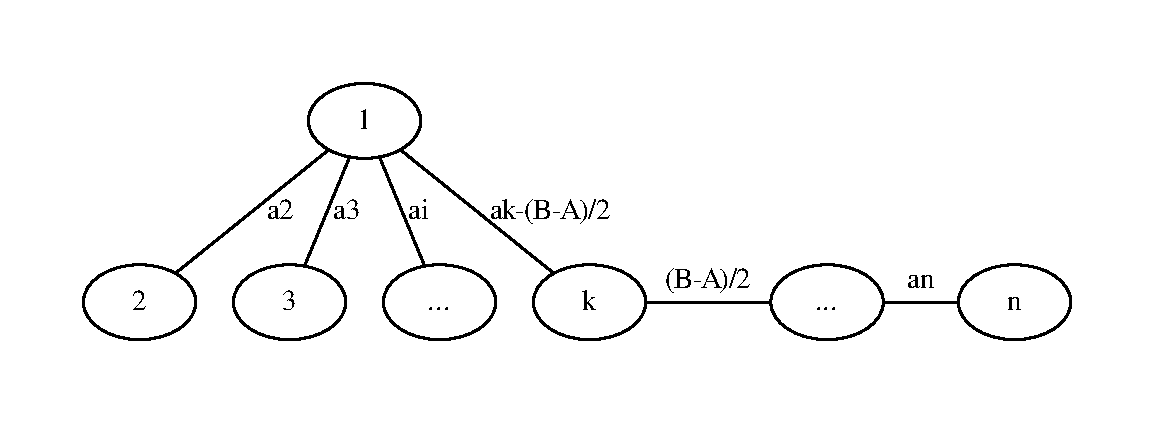
\includegraphics[width=0.5\textwidth]{figures/7-5.pdf}
\end{center}

    Therefore, we can construct a Weighted Graph if $a_1 \leq a_2 + \dots + a_n$.


    \end{proof}
\end{exercise}



\paragraph{Allowing negative edge weights.} Suppose now we allow negative edge weights, like here:
\begin{center}
  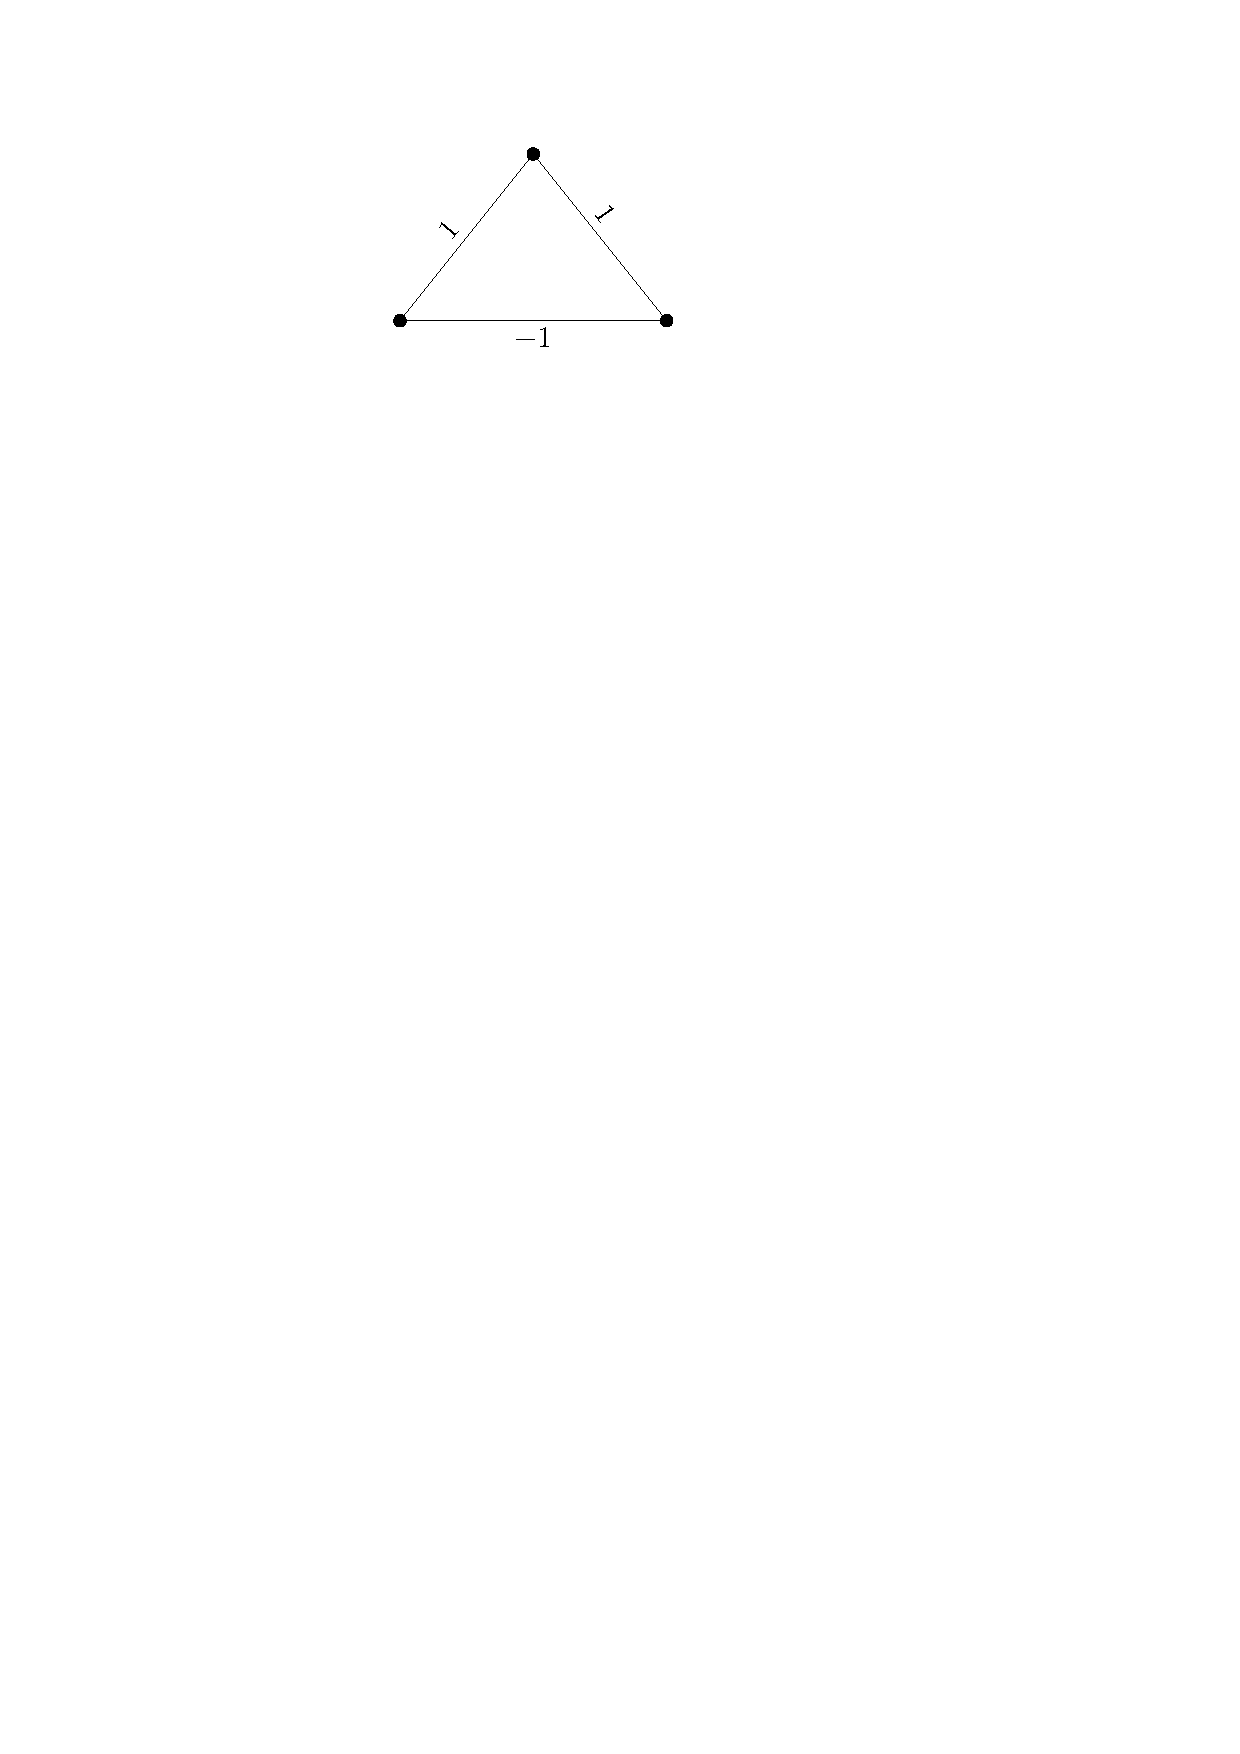
\includegraphics[width=0.25\textwidth]{figures/arbitrary-weighted-graph-score.pdf}
\end{center}
This ``graph with real edge weights'' has score $(2,0,0)$. This score is impossible for
graphs, multigraphs, and weighted graphs with non-negative edge weights.


\begin{exercise}
  State a score theorem for weighted graphs when we allow
  negative edge weights. That is, state a theorem like
  \begin{theorem}[Score Theorem for Graphs with Real Edge Weights]
     Let $(a_1,\dots,a_n) \in \R^n$. There is a  graph with real edge weights
     with this score if and only if $n \geq 3$ or $a_1 = a_2$ when $n=2$ or $a_1 = 0$ when $n=1$.
  \end{theorem}  
\end{exercise}

\begin{exercise}
Prove your theorem.
    \begin{proof}

        Obviously, if there is a graph with real edge weights, $n \geq 3$ or $a_1 = a_2$ when $n=2$ or $a_1 = 0$ when $n=1$.

        Suppose $v_1, v_2 , \dots, v_n$ are the corresponding vertices of $a_1, a_2, \dots, a_n$.

        When $n=1$, obviously, there is a graph with real edge weights if and only if $a_1=0$.

        When $n=2$, obviously, there is a graph with real edge weights if and only if $a_1=a_2$.

        When $n=3$, suppose $x, y, z$ be the weight of $E(v_2, v_3), E(v_1, v_3), E(v_1, v_2)$.

        According to the degree of each vertices, there are equations as followings:
        $$
        \begin{cases}
            x + y = a_3 \\
            x + z = a_2 \\
            y + z = a_1
        \end{cases}
        $$

        The solution is:
        $$
        \begin{cases}
            x = \frac{a_2 + a_3 - a_1}{2} \\
            y = \frac{a_1 + a_3 - a_2}{2} \\
            z = \frac{a_1 + a_2 - a_3}{2}
        \end{cases}
        $$

        Therefore, for every sequence $a_1, a_2, a_3$, there is a graph with real edge weights.

        When $n \geq 4$.

        Connect an edge of weight $a_i$ between $v_i$ and $v_1$, $i \geq 4$.

        Now we can image $v_1, v_4, \dots, v_n$ as a "big" vertice $v_1^\prime$. To promise the degree of $v_1$, the degree of the "big" vertice is $a_1^\prime = a_1 - a_4 - \dots - a_n$.

        In fact, it becomes the cases that $n=3$.
        Suppose $x, y, z$ be the weight of $E(v_2, v_3), E(v_1^\prime, v_3), E(v_1^\prime, v_2)$.

        $$
        \begin{cases}
            x + y = a_3 \\
            x + z = a_2 \\
            y + z = a_1^\prime
        \end{cases}
        $$

        $$
        \begin{cases}
            x = \frac{a_2 + a_3 - a_1^\prime}{2} \\
            y = \frac{a_1^\prime + a_3 - a_2}{2} \\
            z = \frac{a_1^\prime + a_2 - a_3}{2}
        \end{cases}
        $$

\begin{center}
  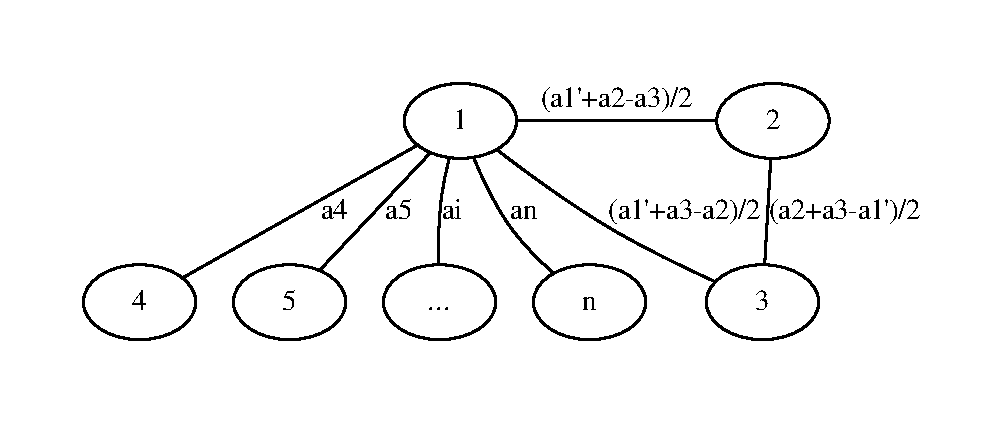
\includegraphics[width=0.5\textwidth]{figures/7-8.pdf}
\end{center}

    Therefore, for $a_1, a_2, \dots, a_n$, $n \geq 4$, there is a graph with real edge weight.

    \end{proof}
\end{exercise}



\begin{exercise}
   For each student ID $(a_1,\dots,a_n)$ in your group, check whether 
   this is (1) a graph score, (2) a multigraph score, (3) a weighted graph score, or
   (4) the score of a graph with real edge weights.
   
   Whenever the answer is {\em yes}, show the graph, when it is {\em no}, 
   give a short argument why. 
\end{exercise}

\paragraph{Example Solution.} My work ID is 50411. 
This is a weighted graph score, as shown by this picture:
\begin{center}
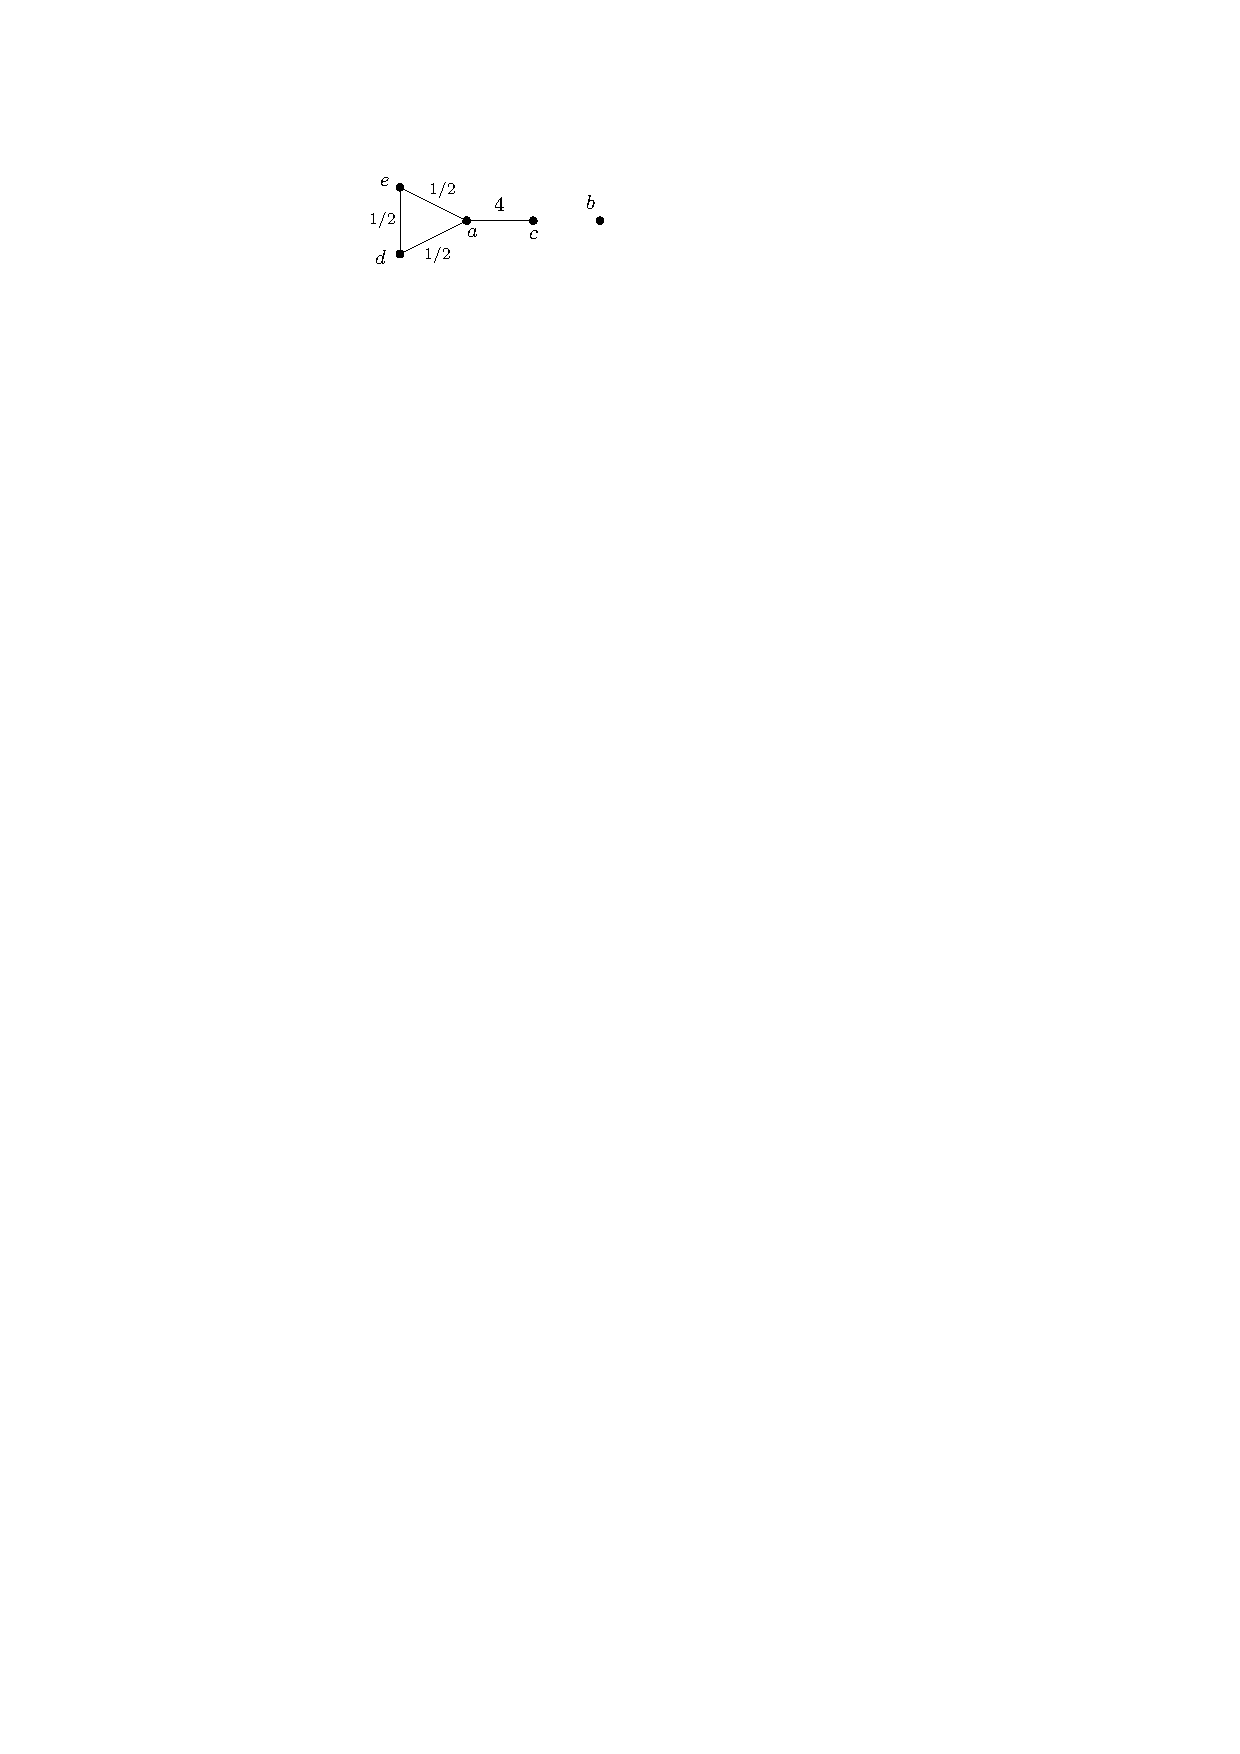
\includegraphics[width=0.4\textwidth]{figures/graph-50411.pdf}
\end{center}
This settles (3). It is not a multigraph score, because BLABLABLA. I won't give more details, as it might
give too many hints about Exercise 7.2. Alright, this settles (2). Note that I do {\em not} need to answer 
(4), as this is already answered by (3). Neither do I need to answer (1), as a ``no'' for (2) implies
a ``no'' for (1).


\paragraph{Solution.} My student ID is 516021910049. 
This is a multigraph score, as shown by this picture:
\begin{center}
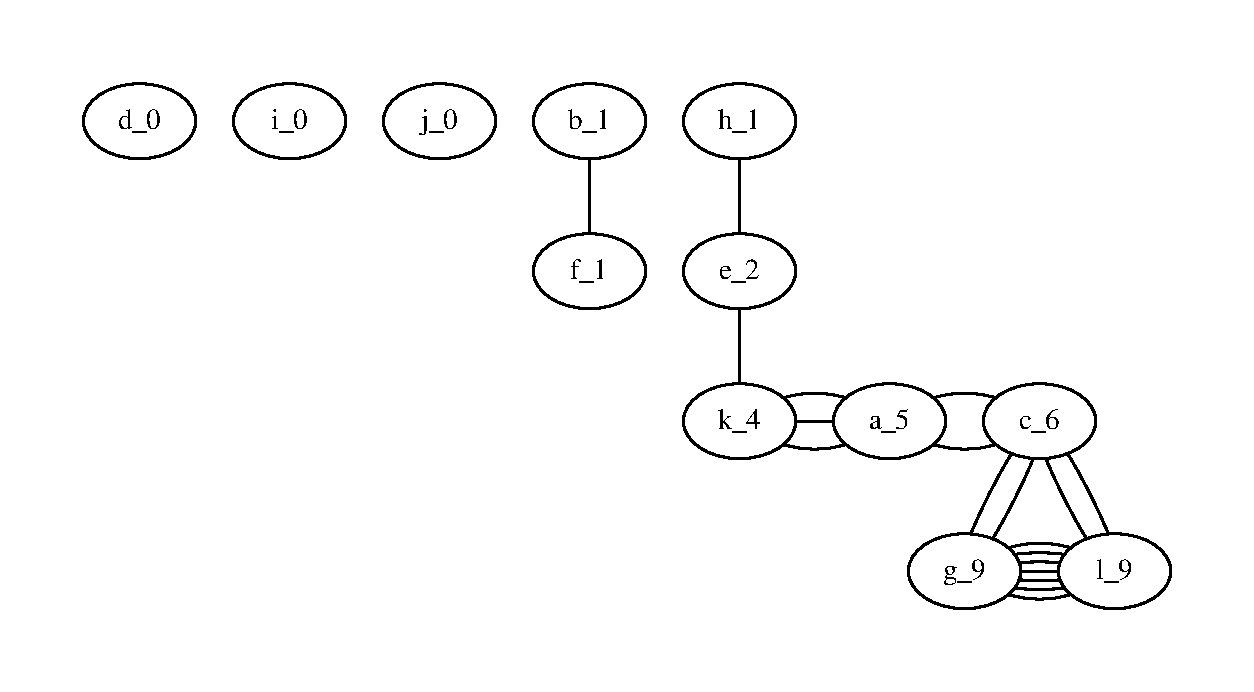
\includegraphics[width=0.6\textwidth]{figures/graph-516021910049.pdf}
\end{center}
This settles (2). It is not a graph score, because there are total 9 non-zero nodes, but the max degree is 9, so no more nodes to satisfy the degree.



\paragraph{Solution.} Ny name is YimingLiu. My student ID is 516021910379.
We sort it in an non-increasing order (997653211100). And we set aside the 2 "0"s so the sequence is d:(9976532111)
\par It is not a graph score because d':(865421000) is not a score.
\par It is a multigraph score because the sum of degrees is an even number and the largest degree of the vertices is smaller than the sum of other degree of other vertices. As is shown in the picture:
\par It is a weighted graph score. As is shown in the picture:
\par It is the score of a graph with real edge weights. As is shown in the picture:
\begin{center}
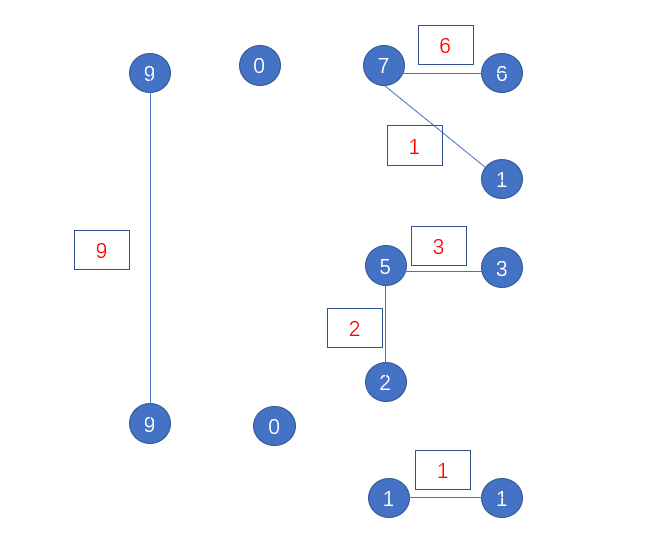
\includegraphics[width=0.4\textwidth]{lym1.png}
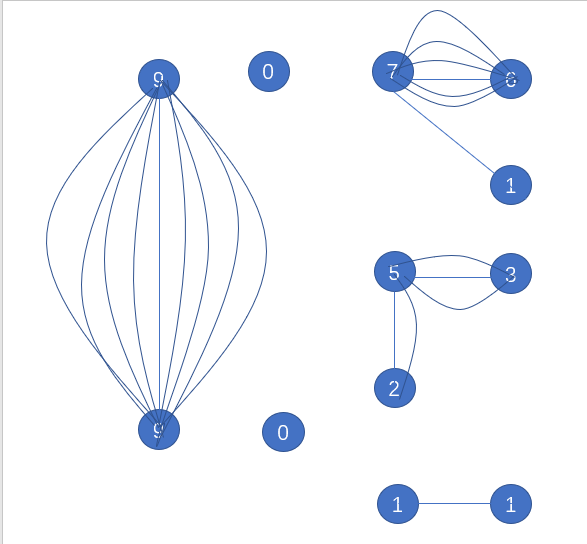
\includegraphics[width=0.4\textwidth]{lym2.png}
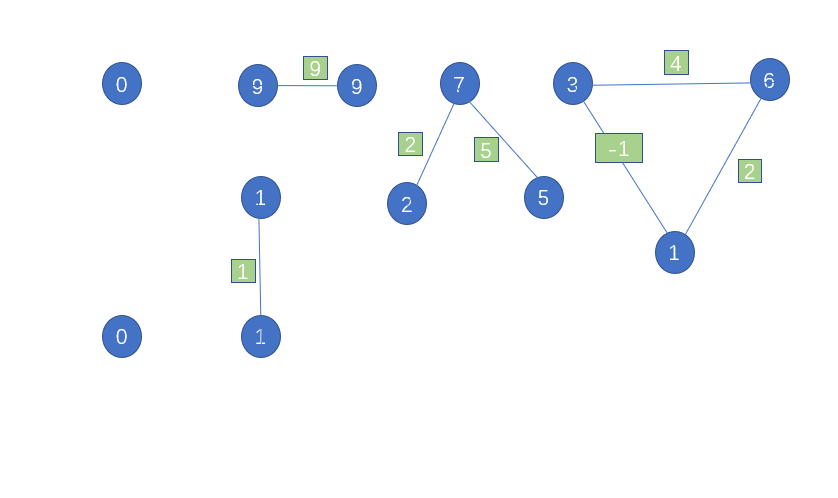
\includegraphics[width=0.4\textwidth]{lym3.png}
\end{center}

I'm Zhou Yiyuan, my student ID is 516021910270. This is a multigraph score, as shown by this picture:\\
\begin{center}
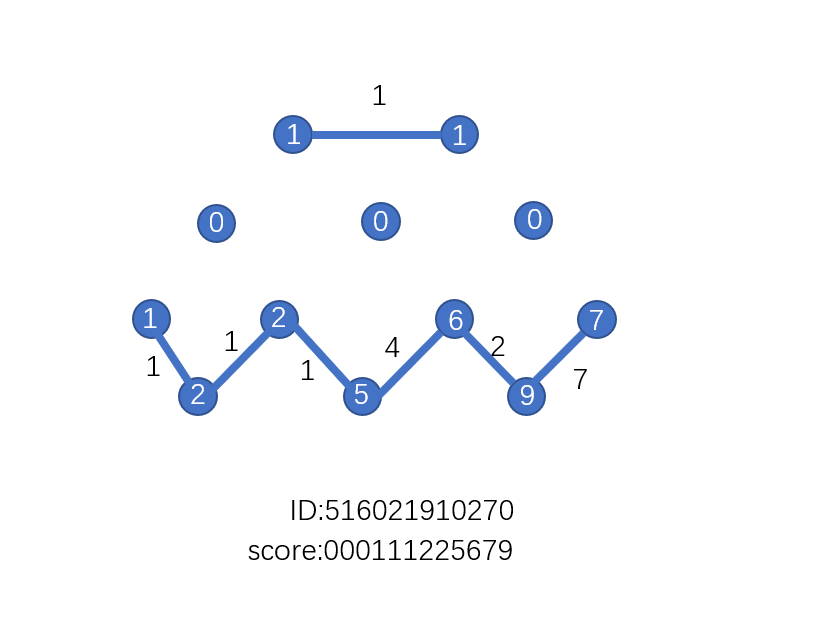
\includegraphics[width=0.4\textwidth]{7-11zyy.png}
\end{center}
 This settles(2). It's not a graph score, because the score of my ID is (000111225679), and the largest degree is 9, which is larger than 8, the quantity of verticals with a non-zero degree except the largest one.


\end{document}
